\chapter{Requisitos do Sistema}
Os requisitos são capacidades que devem ser atendidas ou possuídas por um sistema para resolver um problema ou atingir um objetivo, O conjunto de todos os requisitos que formam a base para o desenvolvimento subsequente de um software \cite{vazquez2016}. Neles são definidos como serão os comportamentos do sistema e seus fluxos. Eles serão abordados em dois segmentos: Os Requisitos funcionais que são fluxos do sistema e os requisitos não funcionais que são necessários para a utilização do sistema.

\section{Requisitos Funcionais}

{ Conforme \cite{essi2005}, requisitos funcionais são as necessidades descritas pelo cliente, onde a equipe do projeto analisa e
especifica as funções, desempenho, interfaces e restrições, conforme as fases das metodologias aplicadas. Sua finalidade é disntringuir as dependências do sistema para que o mesmo funcione de acordo com os requisitos informados pelo cliente. }

\subsection{Cadastros}


\begin{subalineas}
	\item {Usuários};
	\item {Setores};
	\item {Máquinas};
	\item {Unidades de medida};
	\item {Peças};
	\item {Tipos de estoques};
	\item {Estoque de peças};
	\item {Ordem de manutenção}.
\end{subalineas}

\subsection{Consultas}
\begin{subalineas}
	\item {Máquinas};
	\item {Estoque de peças};
	\item {Ordem de manutenção};
	\item {Login};
	\item {Logoff}.
\end{subalineas}

\subsection{Funcionalidades}
\begin{subalineas}
	\item {Monitor de ordens em aberto};
	\item {Solicitação de abertura de ordem de manutenção};
	\item {Central de notificação}.
\end{subalineas}

\section{Requisitos Não Funcionais}

{\cite{IIBA2005} relata que o propósito dos requisitos não funcionais é descrever as qualidades requeridas para um sistema, como sua usabilidade e seu desempenho. Em sistemas alguns destes requisitos podem determinar tecnologias ou algoritmos específicos a serem utilizados, garantindo compatibilidade com sistemas existentes \cite{cordeiro2007}

\subsection{Funcionalidades}
\begin{subalineas}
	\item {Sistema desenvolvido para web};
	\item {Utilizar o banco MS Sql Server};
	\item {Usuários devem ter acesso à computadores e/ou dispositivos móveis}.
\end{subalineas}

\section{Fluxograma do Sistema Desenvolvido}

{Segundo \cite{pejeronimo2002} fluxograma é uma representação gráfica das tarefas de um determinado processo, sendo de forma sequencial a execução delas. \cite{roberthurt} relata que um fluxograma fornece um panorama de alto nível sobre um sistema de informação.

\newpage
\begin{figure}[htb]
	\caption{\label{flux_sys}Fluxo do AGIL.IT}
	\begin{center}
		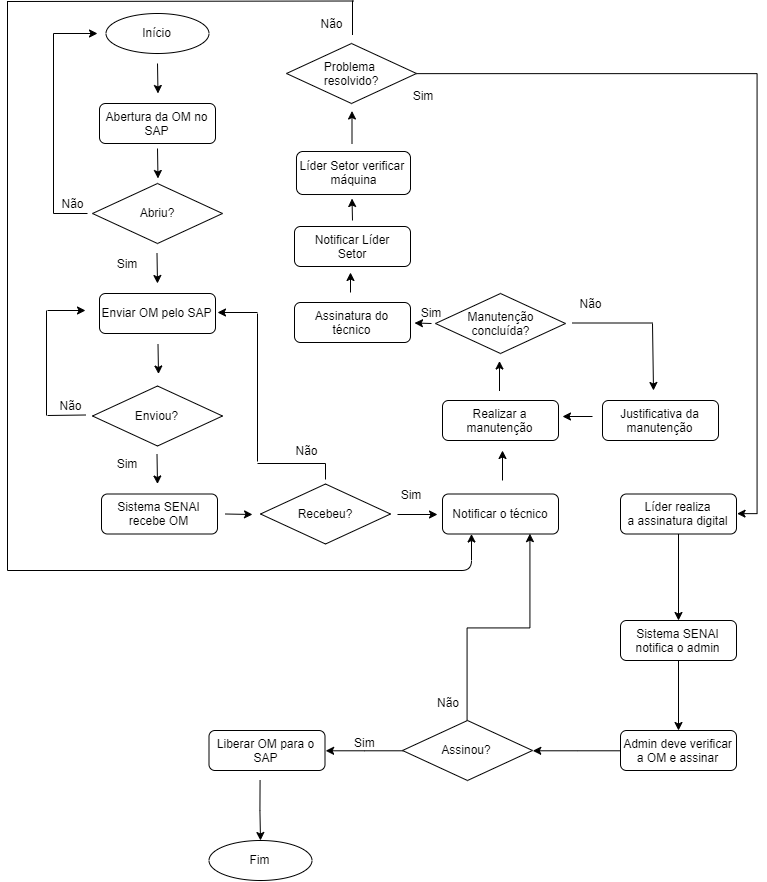
\includegraphics[scale=0.55]{./Figuras/fluxo-sistema.png}
	\end{center}
	\legend{Fonte: Próprio Autor, 2019}
\end{figure}

Na Figura \ref{flux_sys} é possível verificar todo o fluxo do sistema onde começa e termina com a integração do SAP.
O sistema irá receber a OM do SAP e notificar o técnico. Após o técnico realizar a manutenção os usuários realizam as assinaturas e o usuário administrador analisa e libera a OM para a integração.


\section{Diagrama de Caso de Uso do Sistema }

{Diagramas dos casos de uso são técnicas utilizadas para captar os requisitos funcionais de um sistema, descrevem as interações entre usuários de um sistema e o próprio sistema, fornecendo uma narrativa sobre como ele é utilizado \cite{umlessencial2005}. Para \cite{carniello2003} seu objetivo principal consiste em definir o comportamento de um sistema, sem revelar sua estrutura interna.}

\newpage
\begin{figure}[htb]
	\caption{\label{caso_uso}Caso de Uso do AGIL.IT}
	\begin{center}
		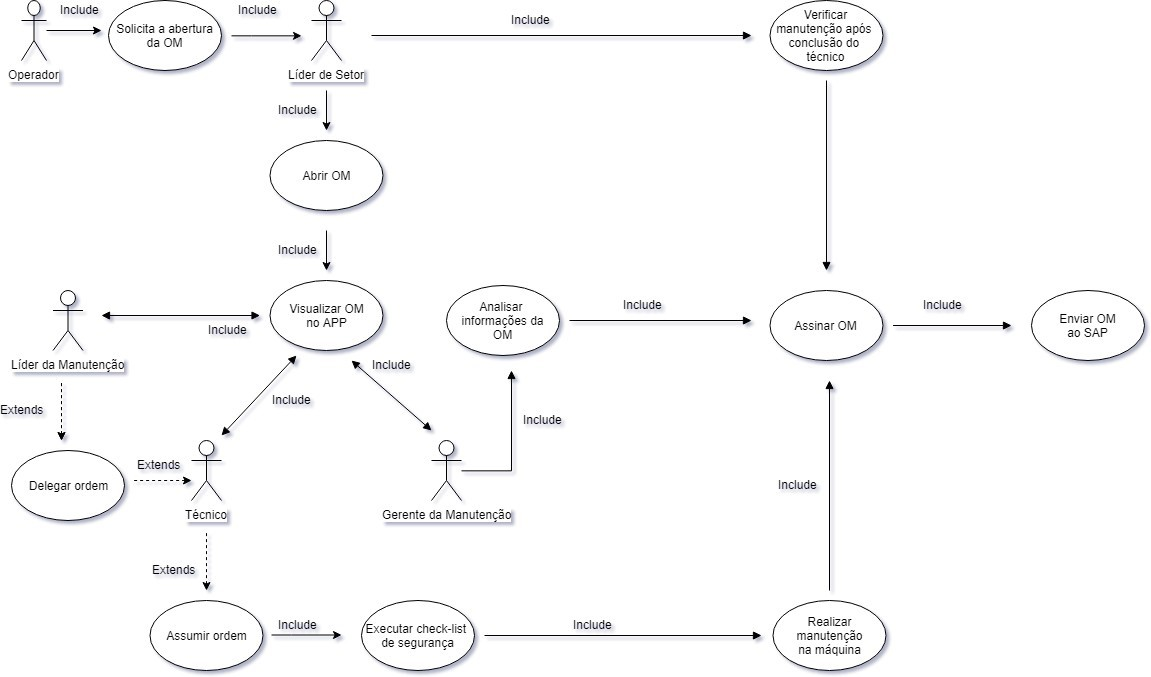
\includegraphics[scale=0.50]{./Figuras/caso-uso.png}
	\end{center}
	\legend{Fonte: Próprio Autor, 2019}
\end{figure}

Na Figura \ref{caso_uso} é possível verificar quais ações cada ator desempenhará no sistema.
Os operadores de máquinas e os líderes de manutenção verificam a manutenção feita e assinam a OM. O técnico realizará a manutenção e verificará as peças necessárias para realizar a assistência ao equipamento e se as mesmas possuem estoque disponível. E o administrador realizará cadastros e encerará as ordens de manutenção.


\section{Entidade de Relacionamento do Banco de Dados}

{Planejar todas as etapas, dedicando a atenção especialmente ao projeto de estruturação do banco de dados. Com a estrutura pronta, a facilidade para dar manutenção no sistema fica muito mais fácil.
Tem como objetivo, obter uma descrição de forma abstrata dos dados que serão armazenados no banco de dados \cite{2010_erbd}. }


\newpage
\begin{figure}[htb]
	\caption{\label{entidade_relacionamento}Entidade de Relacionamento}
	\begin{center}
		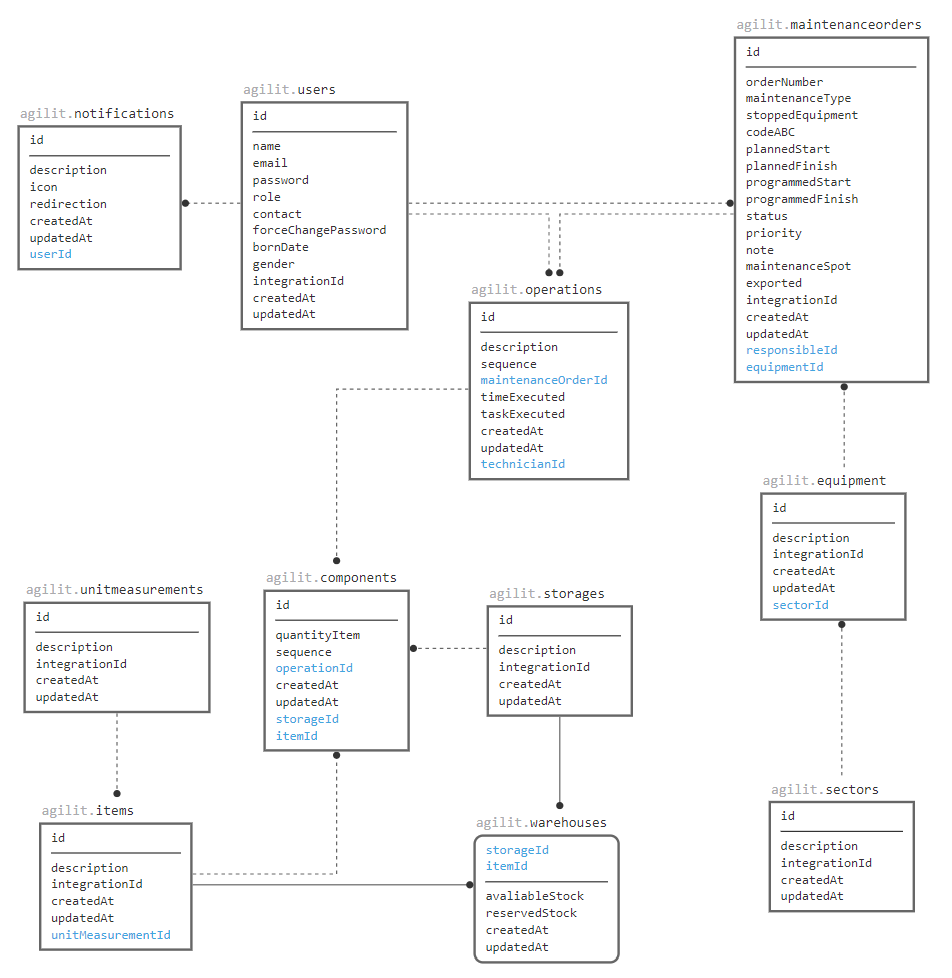
\includegraphics[scale=0.70]{./Figuras/er3.png}
	\end{center}
	\legend{Fonte: Próprio Autor, 2019}
\end{figure}

A Figura \ref{entidade_relacionamento} mostra toda a entidade de relacionamento do banco de dados, onde cada tabela representa uma estrutura de dados no banco de dados e as ligações entre elas demonstram relacionamentos que essas tabelas possuem entre si.


\newpage
\section{Cronograma do Projeto}


Todo bom projeto deve ter um cronograma e um planejamento de ação, baseado nisso, foi elaborado dois cronogramas: um apresentando todo o conteúdo aprendido no semestre e outro montando plano de ação para implementação do projeto.

As figuras a seguir, são cronogramas que demonstram a trajetória do desenvolvimento do projeto. Divididos por semestre, os cronogramas listam as atividades aprendidas nas UCs, com todas as partes teóricas e práticas onde o objetivo principal é implementar todo conhecimento adquirido em prol de um projeto único: A unificação de todas as UCs do curso de Sistemas para Internet.

\begin{figure}[htb]
	\caption{\label{cron-3-semestre}Cronograma de Aprendizagem: Terceiro Semestre}
	\begin{center}
		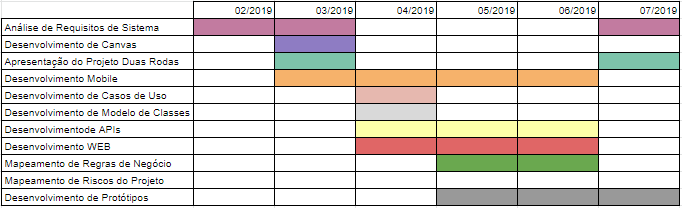
\includegraphics[scale=0.90]{./Figuras/cronograma-3-semestre.png}
	\end{center}
\end{figure}


\begin{figure}[htb]
	\caption{\label{cron-4-semestre}Cronograma de Aprendizagem: Quarto Semestre}
	\begin{center}
		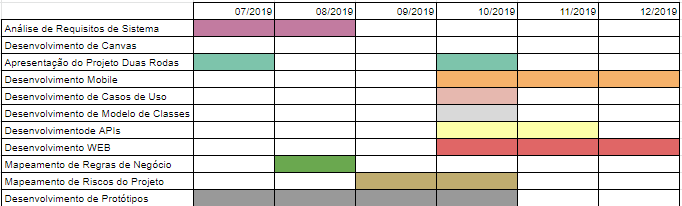
\includegraphics[scale=0.90]{./Figuras/cronograma-4-semestre.png}
	\end{center}
\end{figure}


\begin{figure}[htb]
	\caption{\label{cron-4-semestre}Cronograma de Aprendizagem: Quinto Semestre}
	\begin{center}
		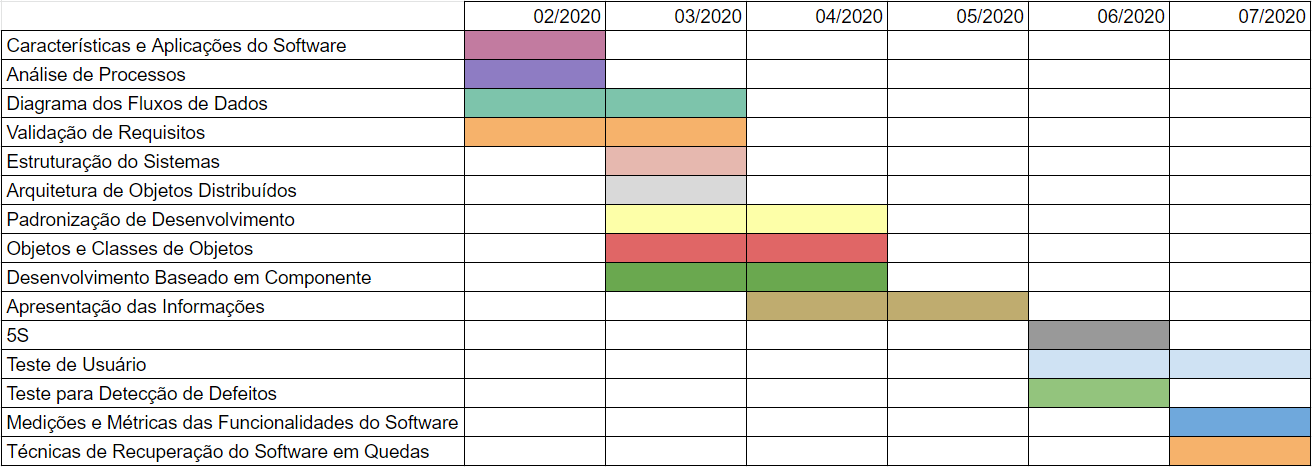
\includegraphics[scale=0.70]{./Figuras/cronograma-5-semestre.png}
	\end{center}
\end{figure}